% !TEX root = ../teoria.root.tex

\documentclass[../teoria.root.tex]{subfiles}

\begin{document}
\section{Límites y Continuidad}
\subsection{Límite de funciones}
En lo que sigue, veremos cómo la noción de límite introducida para sucesiones se extiende al caso de funciones reales.
Esto nos permitirá estudiar el comportamiento de una función \(f\) ”en el infinito” (es decir, los valores \(f(x)\) para \(x\) ”grandes” en valor absoluto) y en los ”bordes” de su dominio de definición, de manera de obtener información útil para la construcción del gráfico de \(f\).
\subsubsection{Límites en el infinito - Asíntotas horizontales}
Consideremos la función \(f\) cuyo gráfico es el siguiente:
\begin{center}
	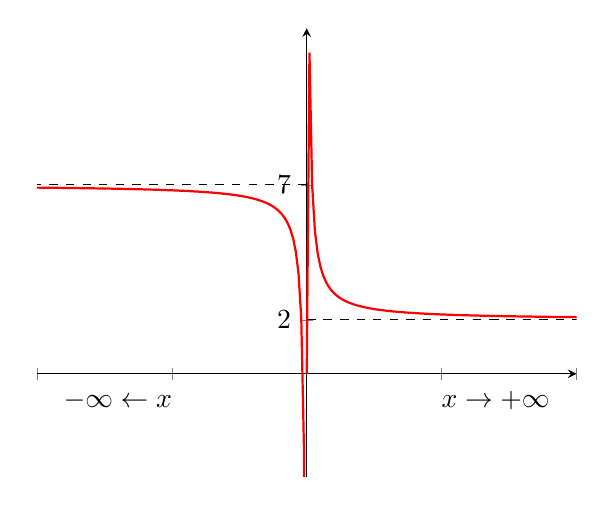
\begin{tikzpicture}[
			declare function={
					f(\x)=(\x<0) * ((7*\x+1)/(\x)) +
					(0<\x) * ((2*\x+1)/(\x));
				}
		]
		\begin{axis}[
				axis lines = middle,
				axis equal,
				xticklabels={,,},
				ytick={2,7},
				samples= 100,
				ymax=8,
				ymin=1
			]
			\foreach \xStart/\xEnd  in {-10/0, 0/10} {
					\addplot[thick,domain=\xStart:\xEnd, red, samples=100] {f(x)};
				}
			\addplot[dashed,domain=0:10] {2};
			\addplot[dashed,domain=0:-10] {7};
			\draw (7,-1) node{\(x\rightarrow+\infty\)};
			\draw (-7,-1) node{\(-\infty\leftarrow x\)};
		\end{axis}
	\end{tikzpicture}
\end{center}
Cuando \(x\) toma valores positivos muy grandes, \(f(x)\) toma valores cercanos a 2;
más precisamente, los valores de \(f(x)\) se acercan tanto como se desee a 2 si se consideran valores de \(x\) positivos suficientemente grandes.
Se dice, entonces, que \(f\) tiende a 2 cuando \(x\) tiende a más infinito o que el límite cuando \(x\) tiende a más infinito de \(f(x)\) es 2, y se nota:
\[\lim_{x\to+\infty}f(x)=2\]
Además, se dice que la recta de ecuación \(y=2\) es una asíntota horizontal para \(f\).

Por otra parte, cuando \(x\) toma valores negativos suficientemente grandes en valor absoluto, \(f\) toma valores tan cercanos a 7 como se quiera;
es decir, el límite cuando \(x\) tiende a menos infinito de \(f(x)\) es 7.
Esto se nota:
\[\lim_{x\to-\infty}f(x)=7\]
En este caso, se dice también que la recta de ecuación \(y=7\) es una asíntota horizontal para \(f\).

Para la función \(g\) cuyo gráfico es
\begin{center}
	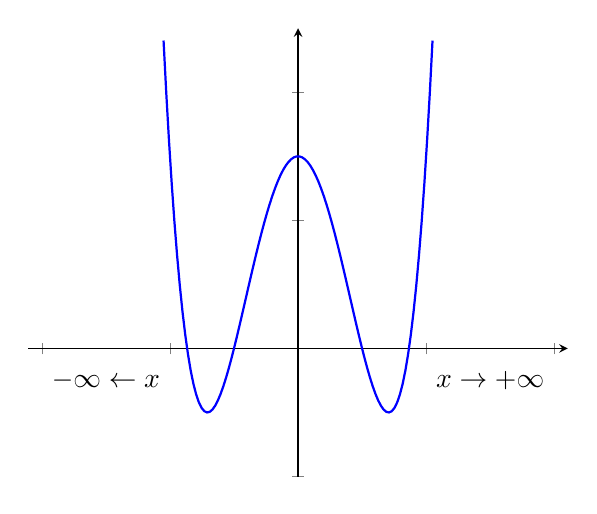
\begin{tikzpicture}
		\begin{axis}[
				axis lines = middle,
				axis equal,
				yticklabels={,,},
				xticklabels={,,},
				samples= 100,
				ymax=5,
				ymin=-2
			]
			\addplot[thick,domain=-2.1:2.1, blue, samples=100] {x^4-4*x^2+3};
			\draw (3,-.5) node{\(x\rightarrow+\infty\)};
			\draw (-3,-.5) node{\(-\infty\leftarrow x\)};
		\end{axis}
	\end{tikzpicture}
\end{center}
tenemos que, cuando \(x\) tiende a más infinito y a menos infinito, \(g(x)\) toma valores arbitrariamente grandes, es decir:
\[\lim_{x\to-\infty}g(x)=+\infty\quad\text{y}\quad\lim_{x\to+\infty}g(x)=+\infty\]
En este caso, no hay asíntotas horizontales.

Finalmente, consideremos la función \(h\) cuyo gráfico es el siguiente:
\begin{center}
	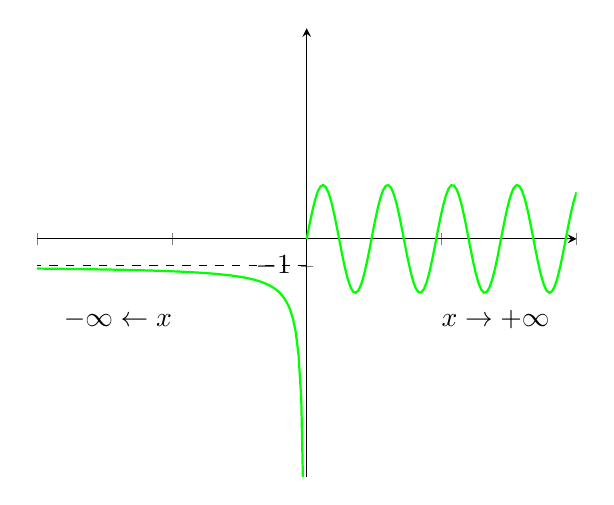
\begin{tikzpicture}[
			declare function={
					f(\x)=(\x<0) * ((-\x+1)/(\x)) +
					(0<\x) * (2*sin(150*\x));
				}
		]
		\begin{axis}[
				axis lines = middle,
				axis equal,
				xticklabels={,,},
				ytick={-1},
				samples= 100,
				ymax=2,
				ymin=-3
			]
			\foreach \xStart/\xEnd  in {-10/0, 0/10} {
					\addplot[thick,domain=\xStart:\xEnd, green, samples=100] {f(x)};
				}
			\addplot[dashed,domain=0:-10] {-1};
			\draw (7,-3) node{\(x\rightarrow+\infty\)};
			\draw (-7,-3) node{\(-\infty\leftarrow x\)};
		\end{axis}
	\end{tikzpicture}
\end{center}
Aunque tenemos que
\[\lim_{x\to-\infty}h(x)=-1,\]
cuando analizamos el límite cuando \(x\) tiende a más infinito, no ocurre ninguna de las situaciones que hemos visto:
los valores de \(h(x)\) no se acercan a ningún número particular ni se van a más o menos infinito;
por lo tanto, no existe \(\lim_{x\to+\infty}h(x)\).
Para esta función, la recta de la ecuación \(y=−1\) es asíntota horizontal.
\subsubsection{Límite en un punto - Asíntotas verticales}
Consideremos la función \(f\) cuyo gráfico es el siguiente:
\begin{center}
	\begin{tikzpicture}[
			declare function={
					f(\x)=(\x<1) * ((\x-2)/(\x-1)) +
					(1<\x) * ((2*\x-1)/(-\x+1)+4);
				}
		]
		\begin{axis}[
				axis lines = middle,
				axis equal,
				yticklabels={,,},
				xticklabels={,,},
				samples= 100,
				ymax=3,
				ymin=-1
			]
			\foreach \xStart/\xEnd  in {-3/1, 1/3} {
					\addplot[thick,domain=\xStart:\xEnd, red, samples=100] {f(x)};
				}
			\draw[dashed] (1,-1.5) -- (1,3.5);
			\draw (.8,-0.5) node{1};
			\draw (0,0.2) node{\(x\to1^-\)};
			\draw (2,0.2) node{\(1^+\leftarrow x\)};
		\end{axis}
	\end{tikzpicture}
\end{center}
Observamos que, cuando \(x\) se acerca a 1 por la izquierda (es decir, considerando sólo valores \(x\) tales que \(x<1\)), la función toma valores positivos arbitrariamente grandes.
En este caso, decimos que el límite de \(f(x)\) cuando \(x\) tiende a 1 por izquierda es \(+\infty\) y escribimos:
\[\lim_{x\to1^-}f(x)=+\infty\]
(el signo - en 1- indica que la variable se acerca a 1 por izquierda).

Asimismo, a medida que \(x\) se acerca a 1 por la derecha (es decir, considerando sólo valores \(x\) tales que \(x>1\)), la función toma valores negativos arbitrariamente grandes en valor absoluto.
En este caso, decimos que el límite de \(f(x)\) cuando \(x\) tiende a 1 por derecha es \(-\infty\) y escribimos:
\[\lim_{x\to1^+}f(x)=-\infty\]
(el signo \(+\) en \(1^+\) indica que la variable se acerca a 1 por derecha).

Consideremos ahora la función \(g\) cuyo gráfico es el siguiente:
\begin{center}
	\begin{tikzpicture}[
			declare function={
					f(\x)=(\x<1) * ((\x+0.1)/(\x-1)+2) +
					(1<\x) * (x+1);
				}
		]
		\begin{axis}[
				axis lines = middle,
				axis equal,
				ytick={2},
				xticklabels={,,},
				samples= 100,
				ymax=4,
				ymin=-1
			]
			\foreach \xStart/\xEnd  in {-3/1, 1/3} {
					\addplot[thick,domain=\xStart:\xEnd, blue, samples=100] {f(x)};
				}
			\draw[dashed] (1,-1.5) -- (1,4.5);
			\addplot[dashed,domain=0:1] {2};
			\draw (1.2,-0.5) node{1};
			\draw (0,0.2) node{\(x\to1^-\)};
			\draw (2,0.2) node{\(1^+\leftarrow x\)};
		\end{axis}
	\end{tikzpicture}
\end{center}
De manera similar al ejemplo anterior, observamos en el gráfico que, cuando \(x\) se acerca a 1 por la izquierda, la función \(g\) toma valores negativos que se hacen tan grandes en valor absoluto como uno quiera con tal que \(x\) esté suficientemente cerca de 1.
Entonces:
\[\lim_{x\to1^-}g(x)=-\infty\]
En cambio, cuando \(x\) se acerca a 1 por la derecha, vemos que los valores de \(g(x)\) se hacen tan cercanos al número 2 como se quiera.
Decimos entonces que el límite de \(g(x)\) cuando \(x\) tiende a 1 por la derecha es 2 y escribimos:
\[\lim_{x\to1^+}g(x)=2\]
Si el límite de una función, cuando \(x\) tiende a un valor \(x_0\) por izquierda, da infinito (\(+\infty\) o \(-\infty\)), o bien el límite cuando \(x\) tiende a \(x_0\) por derecha da infinito, o si se dan ambas situaciones simultáneamente, se dice que la recta \(x=x_0\) es una asíntota vertical.
Por ejemplo, las funciones \(f\) y \(g\) de los gráficos de arriba tienen como asíntota vertical a la recta de ecuación \(x=1\) (si bien \(\lim_{x\to1^+}g(x)=2\) no es infinito, alcanza con que \(\lim_{x\to1^−}g(x)=-\infty\) para afirmar que \(x=1\) es asíntota vertical para \(g\)).

Los límites por derecha y por izquierda no necesariamente deben dar distinto, o infinito.
Por ejemplo, en la función \(h\) del siguiente gráfico
\begin{center}
	\begin{tikzpicture}
		\begin{axis}[
				axis lines = middle,
				axis equal,
				ytick={4},
				yticklabels={\(y_0\)},
				xticklabels={,,},
				samples= 100,
				ymax=7,
				ymin=-1
			]
			\foreach \xStart/\xEnd  in {-.5/1, 1/4} {
					\addplot[thick,domain=\xStart:\xEnd, blue, samples=100] {x^2-2*x+1};
				}
			\draw[dashed] (3,0) -- (3,4);
			\draw (3,-0.5) node{\(x_0\)};
			\node[draw,shape=circle,fill=black,scale=0.4] at (3,4){};
			\addplot[dashed,domain=0:3] {4};
		\end{axis}
	\end{tikzpicture}
\end{center}
vemos que dado un valor \(x_0\), si \(x\) está suficientemente cerca de \(x_0\) (ya sea a la derecha o a la izquierda), los valores de \(h(x)\) están arbitrariamente cerca del número \(y_0=h(x_0)\).
Decimos, entonces, que el límite de \(h(x)\) cuando \(x\) tiende a \(x_0\) es \(y_0\) y escribimos:
\[\lim_{x\to x_0}h(x)=y_0\]
(la notación \(x\to x_0\) significa que \(x\) se acerca a \(x_0\) tanto por la derecha como por la izquierda).
\subsubsection{Límites especiales}
Estudiaremos ahora dos límites especiales que utilizaremos como base para el cálculo de otros límites.

En primer lugar, consideraremos el siguiente límite:
\[\lim_{x\to0}\frac{\sin(x)}{x}\]
Dado que \(\lim_{x\to0}\frac{\sin(x)}{x}\), se trata de una indeterminación del tipo \(\frac{0}{0}\).
Mediante el siguiente razonamiento geométrico, se deduce que vale:
\[\lim_{x\to0}\frac{\sin(x)}{x}=1\]
Más aún, si hacemos un cambio de variables para reducirlo al caso anterior, resulta que:
Si \(f\) es una función tal que \(\lim_{x\to a}f(x)=0\), entonces \(\lim_{x\to a}\frac{\sin(f(x))}{f(x)}=1\).

Para deducir el valor de este límite, utilizaremos una visualización geométrica.
Consideremos un ángulo de \(x\) radianes (con \(0<x<\frac{\pi}{2}\)) con vértice en el origen de coordenadas \(O\), un lado sobre el eje de las abscisas y el otro, en el primer cuadrante.
Los lados de este ángulo intersecan a la circunferencia de radio 1 en dos puntos, \(P\) y \(Q\), determinando un sector circular \(POQ\).
Construimos dos triángulos rectángulos, \(OAP\) y \(OQB\), como se muestra en la figura:
\begin{center}
	\begin{scaletikzpicturetowidth}{.5\linewidth}
		\begin{tikzpicture}[scale=\tikzscale]
			\draw[->,thick] (0,-.1) -- (0,1.3);
			\draw[->,thick] (-.1,0) -- (1.3,0);
			\draw[thick] (1,0) arc (0:90:1);
			\draw[thick] (0,0) node[below right]{\(O\)}
			-- (0.87,.5) node[above]{\(P\)}
			-- (.87,0) node[below]{\(A\)}
			-- cycle;
			\draw[thick] (0,0) coordinate (a)
			-- (1,.58) coordinate (b) node[above]{\(B\)}
			-- (1,0) coordinate (c) node[below]{\(Q\)}
			-- cycle pic[pic text=\(x\), draw=red, angle eccentricity=1.5, angle radius=1cm]{angle=c--a--b};
		\end{tikzpicture}
	\end{scaletikzpicturetowidth}
\end{center}
Gráficamente, podemos observar la siguiente relación entre las áreas del sector circular y los dos triángulos rectángulos:
\[\text{área}(\Delta OAP)<\text{área}(POQ)<\text{área}(\Delta OQB)\]
Calculemos estas áreas en función de x:
\begin{itemize}
	\item En el triángulo \(OAP\), tenemos que la medida de su base \(OA\) es \(\cos(x)\), mientras que su altura \(AP\) mide \(\sin(x)\); luego,
	      \[\text{área}(\Delta OAP)=\frac{1}{2}\cos(x)\sin(x)\]
	\item En el triángulo \(OQB\), la base \(OQ\) mide 1 (es el radio de la circunferencia).
	      Para calcular la medida \(h\) de la altura \(QB\), recordemos que el cociente entre las medidas de los dos catetos del triángulo, \(BQ\) y \(OQ\), es \(\tan(x)\);
	      o sea que \(\frac{h}{1}=\tan(x)\).
	      Entonces, \(h=\tan(x)\), y el área del triángulo resulta ser
	      \[\text{área}(\Delta OQB)=\frac{1}{2}\tan(x)=\frac{1}{2}\frac{\sin(x)}{\cos(x)}\]
	\item Finalmente, el área del sector circular es proporcional al ángulo que lo determina y, teniendo en cuenta que el área del círculo (correspondiente a un ángulo de \(2\pi\) radianes) es \(\pi\), resulta que
	      \[\text{área}(POQ)=\frac{x}{2\pi}\pi 1^2=\frac{1}{2}x\]
\end{itemize}
Reemplazando los valores calculados en la desigualdad entre áreas, obtenemos:
\[\frac{1}{2}\cos(x)\sin(x)<\frac{1}{2}x<\frac{1}{2}\frac{\sin(x)}{\cos(x)}\]
Dividiendo cada miembro de la desigualdad anterior por \(\frac{1}{2}\sin(x)>0\), deducimos que
\[\cos(x)<\frac{x}{\sin(x)}<\frac{1}{\cos(x)}\]
y, al considerar los inversos, llegamos a que para \(0<x<\frac{\pi}{2}\) vale:
\[\frac{1}{\cos(x)}<\frac{\sin(x)}{x}<\cos(x)\]
Dado que \(\lim_{x\to0^+}\cos(x)=1\), también vale \(\lim_{x\to0^+}\frac{1}{\cos(x)}=1\) y , entonces, aplicando la propiedad del ”sándwich”, deducimos que
\[\lim_{x\to0^+}\frac{\sin(x)}{x}=1\]
En forma similar, puede verse que
\[\lim_{x\to0^-}\frac{\sin(x)}{x}=1\]
En consecuencia:
\[\lim_{x\to0}\frac{\sin(x)}{x}=1\]
El segundo de los límites especiales que nos interesa calcular es el siguiente:
\[\lim_{x\to+\infty}\left(1+\frac{1}{x}\right)^x\]
Como \(\lim_{x\to+\infty}1+\frac{1}{x}=1\), estamos ante una indeterminación del tipo \(1^\infty\).
Recordemos que, al estudiar sucesiones en la Unidad 2, vimos que
\[\lim_{n\to+\infty}\left(1+\frac{1}{n}\right)^n=e\]
es decir, conocemos el valor del límite cuando la variable \(x\) toma valores en los números naturales en lugar de números reales.
Sin embargo, se puede deducir que también vale:
\[\lim_{x\to+\infty}\left(1+\frac{1}{x}\right)^x=e\]
y que lo mismo ocurre para \(x\to-\infty\), es decir:
\[\lim_{x\to-\infty}\left(1+\frac{1}{x}\right)^x=e\]
A partir de este resultado, es posible calcular otros límites en el caso de indeterminaciones del tipo \(1^\infty\); por ejemplo, calculemos
\[\lim_{x\to0}(1+x)^{\frac{1}{x}}\]
(observemos que, en efecto, se trata de una indeterminación del tipo \(1^\infty\)).
Al hacer el cambio de variable \(y=\frac{1}{x}\), nos queda:
\[\lim_{x\to0}(1+x)^{\frac{1}{x}}=\lim_{y\to\infty}(1+\frac{1}{y})^y=e\]
\subsection{Continuidad}
\end{document}
